% Begin the document and set up the style of the document
\documentclass[a4paper]{article}

% Install the required packages for the document 
\usepackage{envmath}
\usepackage{esvect}
\usepackage{graphicx}
\usepackage{gensymb}
\usepackage{tikz}
\usepackage{geometry}
\usepackage{enumitem}
\usepackage{mathtools}
\usepackage{graphicx}
\usepackage{amsmath}
\usepackage{amscd}
\usepackage{amssymb}
\usepackage{amsfonts}
\usepackage{pgf}
\usepackage{tikz}
\usepackage{mathrsfs}
\usepackage{asyalign}
\usepackage{physics}
\usepackage{cite}
\usepackage{url}
\usepackage[tableposition=top]{caption}
\usepackage{ifthen}
\usepackage[utf8]{inputenc}
\usetikzlibrary{arrows}

\begin{document}

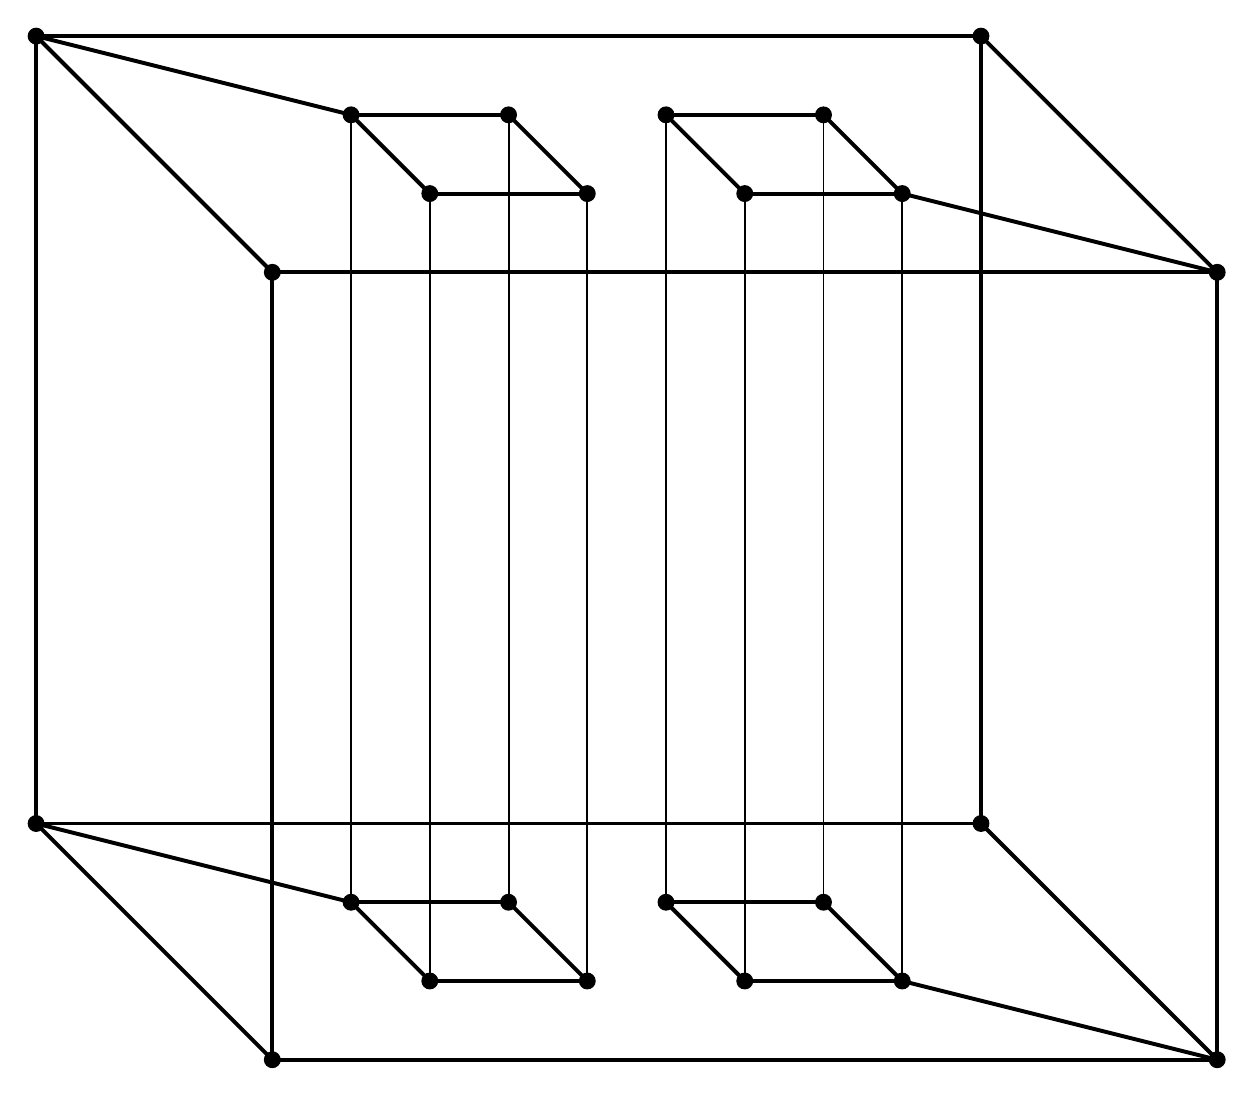
\begin{tikzpicture}

	\draw[line width = 0.5mm] (-3,3) -- (9,3);
	\draw[line width = 0.5mm] (0,0) -- (12,0);
	\draw[line width = 0.5mm] (-3,3) -- (0,0);
	\draw[line width = 0.5mm] (9,3) -- (12,0);
	\draw[line width = 0.5mm] (-3,3) -- (-3,-7);
	\draw[line width = 0.5mm] (0,0) -- (0,-10);
	\draw[line width = 0.5mm] (12,0) -- (12,-10);
	\draw[line width = 0.5mm] (9,3) -- (9,-7);
	\draw[line width = 0.5mm] (-3,-7) -- (9,-7);
	\draw[line width = 0.5mm] (-3,-7) -- (0,-10);
	\draw[line width = 0.5mm] (0,-10) -- (12,-10);
	\draw[line width = 0.5mm] (9,-7) -- (12,-10);

	\draw[line width = 0.5mm] (1,2) -- (3,2);
	\draw[line width = 0.5mm] (1,2) -- (2,1);
	\draw[line width = 0.5mm] (2,1) -- (4,1);
	\draw[line width = 0.5mm] (3,2) -- (4,1);
	\draw[line width = 0.25mm] (1,2) -- (1,-8);
	\draw[line width = 0.25mm] (3,2) -- (3,-8);
	\draw[line width = 0.25mm] (2,1) -- (2,-9);
	\draw[line width = 0.25mm] (4,1) -- (4,-9);
	\draw[line width = 0.5mm] (2,-9) -- (1,-8);
	\draw[line width = 0.5mm] (1,-8) -- (3,-8);
	\draw[line width = 0.5mm] (4,-9) -- (2,-9);
	\draw[line width = 0.5mm] (3,-8) -- (4,-9);

	\draw[line width = 0.5mm] (5,2) -- (7,2);
	\draw[line width = 0.5mm] (5,2) -- (6,1);
	\draw[line width = 0.5mm] (6,1) -- (8,1);
	\draw[line width = 0.5mm] (7,2) -- (8,1);
	\draw[line width = 0.25mm] (5,2) -- (5,-8);
	\draw[line width = 0.25mm] (7,2) -- (7,-8);
	\draw[line width = 0.25mm] (6,1) -- (6,-9);
	\draw[line width = 0.25mm] (8,1) -- (8,-9);
	\draw[line width = 0.5mm] (6,-9) -- (5,-8);
	\draw[line width = 0.5mm] (5,-8) -- (7,-8);
	\draw[line width = 0.5mm] (8,-9) -- (6,-9);
	\draw[line width = 0.5mm] (7,-8) -- (8,-9);

	\draw[line width = 0.5mm] (-3,3) -- (1,2);
	\draw[line width = 0.5mm] (12,0) -- (8,1);
	\draw[line width = 0.5mm] (-3,-7) -- (1,-8);
	\draw[line width = 0.5mm] (12,-10) -- (8,-9);

	\draw[fill] (-3,3) circle (1mm);
	\draw[fill] (9,3) circle (1mm);
	\draw[fill] (0,0) circle (1mm);
	\draw[fill] (12,0) circle (1mm);
	\draw[fill] (-3,-7) circle (1mm);
	\draw[fill] (0,-10) circle (1mm);
	\draw[fill] (12,-10) circle (1mm);
	\draw[fill] (9,-7) circle (1mm);
	\draw[fill] (1,2) circle (1mm);
	\draw[fill] (3,2) circle (1mm);
	\draw[fill] (2,1) circle (1mm);
	\draw[fill] (4,1) circle (1mm);
	\draw[fill] (5,2) circle (1mm);
	\draw[fill] (7,2) circle (1mm);
	\draw[fill] (6,1) circle (1mm);
	\draw[fill] (8,1) circle (1mm);
	\draw[fill] (1,-8) circle (1mm);
	\draw[fill] (3,-8) circle (1mm);
	\draw[fill] (2,-9) circle (1mm);
	\draw[fill] (4,-9) circle (1mm);
	\draw[fill] (5,-8) circle (1mm);
	\draw[fill] (7,-8) circle (1mm);
	\draw[fill] (6,-9) circle (1mm);
	\draw[fill] (8,-9) circle (1mm);


	

\end{tikzpicture}










\end{document}